\documentclass[../chapters.tex]{subfiles}
\begin{document}
    \chapter{Reinforcement Learning}\label{ch:reinforcement-learning}

    In this chapter, we will explore the application of Reinforcement Learning (RL) techniques in the context of portfolio allocation.
    We will begin by providing an overview of RL in context of AI, its fundamental concepts, including the agent, environment, state, action, and reward.
    We will also highlight the motivation for using RL in portfolio allocation and discuss its potential benefits and challenges.
    First we need understand the differences between types of learning:

    \paragraph{Supervised Learning}
    In supervised learning (SL), a model is trained on a labeled dataset, where the input data is paired with corresponding output labels.
    The model learns to make predictions based on the labeled examples, and the goal is to minimize the error between predicted outputs and actual labels.
    Common applications of supervised learning include image classification, speech recognition, and sentiment analysis.

    \paragraph{Semi-supervised Learning}
    Semi-supervised learning (SSL) is a combination of supervised and unsupervised learning.
    It uses a small labeled dataset along with a large unlabeled dataset for training.
    The model leverages the limited labeled examples to learn patterns from the unlabeled data, and then makes predictions on unseen data.
    SSL is useful when obtaining labeled data is expensive or time-consuming.
    It is often used in scenarios where obtaining a large labeled dataset is challenging, such as in medical diagnosis or fraud detection.

    \paragraph{Unsupervised Learning}
    In unsupervised learning (UL), the model learns from unlabeled data without any predefined output labels.
    The goal is to find underlying patterns, structures, or relationships within the data.
    Common unsupervised learning tasks include clustering, dimensionality reduction, and anomaly detection.
    UL is used in scenarios where labeled data is scarce or not available, and the model needs to discover patterns autonomously from the data.

    \paragraph{Reinforcement Learning}
    Reinforcement learning is a type of learning paradigm where an agent interacts with an environment and learns to take actions to maximize a cumulative reward signal~\cite{sutton2018reinforcement}.
    The agent learns through \texttt{trial-and-error}, exploring different actions and receiving feedback in the form of rewards or penalties based on its actions.
    RL is used in scenarios where the optimal action is not known, and the agent needs to learn from feedback to make sequential decisions.
    Common applications of RL include game playing, robotic control, autonomous driving, and financial trading.


    \section{Introduction}\label{sec:rl-introduction}
    Reinforcement learning (RL) is an exciting field at the intersection of artificial intelligence (AI) and machine learning (ML) that deals with training agents to make optimal decisions in dynamic environments.
    RL is inspired by the way humans learn from experience, where an agent interacts with an environment, receives feedback in the form of rewards or penalties, and uses this feedback to learn and improve its decision-making abilities.

    At the heart of RL lies the concept of an agent, which that takes actions in an environment to achieve specific goals.
    The environment is typically modeled as a Markov decision process (MDP), which is a mathematical framework that describes how an agent interacts with an environment in discrete time steps.
    An MDP is defined by a tuple $(S, A, P, R)$, where $S$ is the state space, $A$ is the action space, $P$ is the transition probability function, and $R\in\mathbb{R}$ is the reward.

    The goal of an RL agent is to learn a policy, denoted by $\pi$, which is a mapping from states to actions that maximizes the cumulative rewards over time $T$.
    The agent uses this policy to select actions at each time step, and the environment responds with a new state and a reward.
    The agent then updates its policy based on the observed rewards and states, aiming to improve its decision-making abilities and achieve higher rewards in the long run.

    RL algorithms can be broadly categorized into two main types: model-free and model-based.
    Model-free algorithms are then further divided into value-based and policy-based methods, such as Q-learning (value-based) and policy gradient methods (policy-based), learn directly from the interactions with the environment without explicitly modeling the transition probabilities and rewards.
    Model-based algorithms, on the other hand, learn a model of the environment and use it to make decisions.
    These algorithms have their strengths and weaknesses, and the choice between them depends on the specific problem and requirements.

    The sequence of states, actions and rewards that the agent experiences is called a trajectory, and it look like this:
    \begin{equation}
    (S_0, A_0, R_1, S_1, A_1, R_2, S_2, A_2, \dots, S_{T-1}, A_{T-1}, R_T, S_T)
    \end{equation}

    This sequence of \emph{state-action-reward} can be finite or infinite, depending on the environment and the agent's goal.
    Pretty good example of this is the game of chess, where the game ends when one of the players wins or the game is a draw.
    In this case, the trajectory is finite, and the agent's goal is to maximize the cumulative reward over time $T$.
    On the other hand, the self-driving car example is an infinite-horizon problem, where the agent's goal is to maximize the cumulative reward over an infinite time horizon or until the car reaches its destination.

    \begin{figure}[h!]
        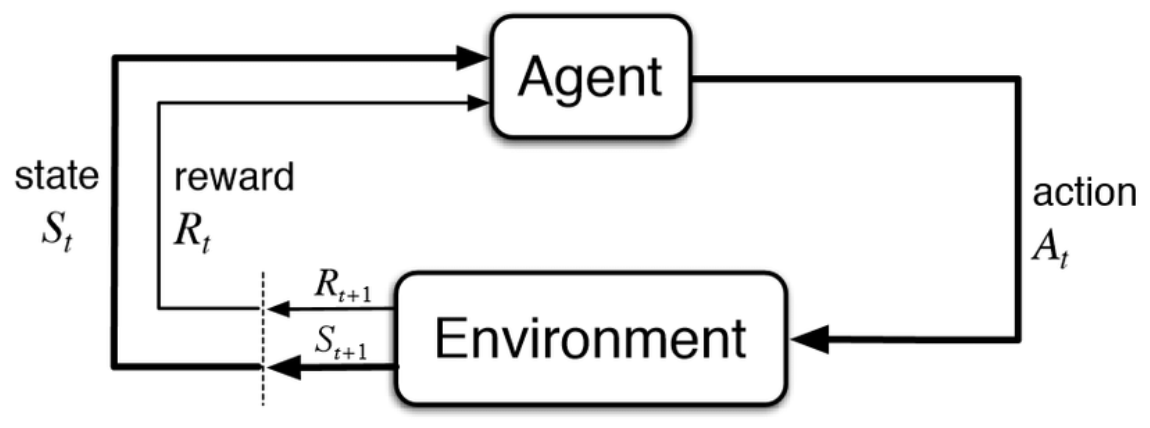
\includegraphics[width=0.8\linewidth]{image/agent-environment}
        \centering
        \caption{The agent interacts with the environment and learns to maximize the cumulative reward over time $T$.}
        \label{fig:rl-introduction}
    \end{figure}


    \section{Markov Models for Reinforcement Learning}\label{sec:markov-models-for-rl}
    TODO

    \subsection{Markov Process}\label{subsec:markov-process}
    TODO

    \subsection{Markov Reward Process}\label{subsec:markov-reward-process}
    TODO

    \subsection{Markov Decision Process}\label{subsec:markov-decision-process}
    TODO

    \subsubsection{State-value Function}\label{subsubsec:state-value-function}
    TODO

    \subsubsection{Action-value Function}\label{subsubsec:action-value-function}
    TODO

    \subsubsection{Stochastic Policy Function}\label{subsubsec:stochastic-policy-function}
    TODO

    \subsubsection{Bellman's Equation}\label{subsec:bellman-equation}
    TODO

    \subsubsection{Bellman's Optimality Equation}\label{subsec:bellman-optimality-equation}
    TODO


    \section{Model-based methods}
    As mentioned in Section~\ref{sec:rl-introduction}, RL algorithms can be broadly categorized into two main types: model-free and model-based.
    Model-based methods rely on \emph{planning} as they primary component, while model-free methods rely on \emph{learning}~\cite{sutton2018reinforcement}.
    One popular approach is to use a probabilistic model of the environment, which can be represented as a transition function $P(s_{t+1}|s_t, a_t)$ that describes the probability of transitioning from state $s_t$ to state $s_{t+1}$ when taking action $a_t$.
    Some popular probabilistic model-based RL methods include Monte Carlo Tree Search, Neural Network Dynamics, and Probabilistic Ensembles with Trajectory Samplin.

    Another approach in model-based RL is to use a learned deterministic model of the environment, which can be represented as a function $f(s_t, a_t)$ that directly maps states and actions to next states.
    Deterministic model-based RL methods, such as World Models, learn an encoder to represent states, a recurrent neural network (RNN) to model dynamics, and a decoder to generate predicted next states.

    \subsection{Advantages and Challenges}

    Model-based RL offers several advantages over model-free methods.
    One major advantage is sample efficiency, as the agent can use the learned model of the environment to plan and generate simulated trajectories for learning, reducing the need for costly real-world interactions.
    Additionally, model-based RL can enable the agent to handle complex, high-dimensional state spaces and long-horizon tasks more effectively.

    However, model-based RL also faces challenges.
    One challenge is the accuracy of the learned model, as any errors in the model can lead to suboptimal policies.
    Another challenge is the computational cost of planning and decision-making using the learned model, as it requires additional computation compared to direct action selection in model-free methods.

    In conclusion, model-based RL is a promising approach that can offer sample-efficient learning and improved performance in complex environments.
    Various methods, such as probabilistic models and deterministic models, have been proposed in the literature.
    Despite some challenges, model-based RL continues to be an active area of research in machine learning.


%\subsection{Value Based Agents}\label{subsec:value-based-agents}


    \section{Value-based methods}
    TODO

    \subsection{Dynamic Programming}\label{subsec:dynamic-programming}
    TODO

    \subsubsection{Policy Iteration}\label{subsubsec:policy-iteration}
    TODO

    \subsubsection{Value Iteration}\label{subsubsec:value-iteration}
    TODO

    \subsection{Monte Carlo Methods}\label{subsec:monte-carlo-methods}
    TODO

    \subsection{Temporal Difference Methods}\label{subsec:temporal-difference-methods}
    TODO

% TODO: Value-based methods for Function Approximation


    \section{Policy-based methods}
    TODO

    \subsection{Policy Gradient Methods}\label{subsec:policy-gradient-methods}
    TODO

    \subsection{Actor-Critic Methods}\label{subsec:actor-critic-methods}
    TODO

    \subsection{Monte Carlo Policy Gradient Methods}\label{subsec:monte-carlo-policy-gradient-methods}
    TODO
\end{document}
